\documentclass[12pt,a4paper]{article}

\usepackage[a4paper,text={16.5cm,25.2cm},centering]{geometry}
\usepackage{lmodern}
\usepackage{amssymb,amsmath}
\usepackage{bm}
\usepackage{graphicx}
\usepackage{microtype}
\usepackage{hyperref}
\usepackage{mhchem}
\setlength{\parindent}{0pt}
\setlength{\parskip}{1.2ex}

\hypersetup
       {   pdfauthor = { Huo Chen },
           pdftitle={ An tutorial on polaron transformed Redfield equation },
           colorlinks=TRUE,
           linkcolor=black,
           citecolor=blue,
           urlcolor=blue
       }

\title{ An tutorial on polaron transformed Redfield equation }

\author{ Huo Chen }


\usepackage{upquote}
\usepackage{listings}
\usepackage{xcolor}
\lstset{
    basicstyle=\ttfamily\footnotesize,
    upquote=true,
    breaklines=true,
    breakindent=0pt,
    keepspaces=true,
    showspaces=false,
    columns=fullflexible,
    showtabs=false,
    showstringspaces=false,
    escapeinside={(*@}{@*)},
    extendedchars=true,
}
\newcommand{\HLJLt}[1]{#1}
\newcommand{\HLJLw}[1]{#1}
\newcommand{\HLJLe}[1]{#1}
\newcommand{\HLJLeB}[1]{#1}
\newcommand{\HLJLo}[1]{#1}
\newcommand{\HLJLk}[1]{\textcolor[RGB]{148,91,176}{\textbf{#1}}}
\newcommand{\HLJLkc}[1]{\textcolor[RGB]{59,151,46}{\textit{#1}}}
\newcommand{\HLJLkd}[1]{\textcolor[RGB]{214,102,97}{\textit{#1}}}
\newcommand{\HLJLkn}[1]{\textcolor[RGB]{148,91,176}{\textbf{#1}}}
\newcommand{\HLJLkp}[1]{\textcolor[RGB]{148,91,176}{\textbf{#1}}}
\newcommand{\HLJLkr}[1]{\textcolor[RGB]{148,91,176}{\textbf{#1}}}
\newcommand{\HLJLkt}[1]{\textcolor[RGB]{148,91,176}{\textbf{#1}}}
\newcommand{\HLJLn}[1]{#1}
\newcommand{\HLJLna}[1]{#1}
\newcommand{\HLJLnb}[1]{#1}
\newcommand{\HLJLnbp}[1]{#1}
\newcommand{\HLJLnc}[1]{#1}
\newcommand{\HLJLncB}[1]{#1}
\newcommand{\HLJLnd}[1]{\textcolor[RGB]{214,102,97}{#1}}
\newcommand{\HLJLne}[1]{#1}
\newcommand{\HLJLneB}[1]{#1}
\newcommand{\HLJLnf}[1]{\textcolor[RGB]{66,102,213}{#1}}
\newcommand{\HLJLnfm}[1]{\textcolor[RGB]{66,102,213}{#1}}
\newcommand{\HLJLnp}[1]{#1}
\newcommand{\HLJLnl}[1]{#1}
\newcommand{\HLJLnn}[1]{#1}
\newcommand{\HLJLno}[1]{#1}
\newcommand{\HLJLnt}[1]{#1}
\newcommand{\HLJLnv}[1]{#1}
\newcommand{\HLJLnvc}[1]{#1}
\newcommand{\HLJLnvg}[1]{#1}
\newcommand{\HLJLnvi}[1]{#1}
\newcommand{\HLJLnvm}[1]{#1}
\newcommand{\HLJLl}[1]{#1}
\newcommand{\HLJLld}[1]{\textcolor[RGB]{148,91,176}{\textit{#1}}}
\newcommand{\HLJLs}[1]{\textcolor[RGB]{201,61,57}{#1}}
\newcommand{\HLJLsa}[1]{\textcolor[RGB]{201,61,57}{#1}}
\newcommand{\HLJLsb}[1]{\textcolor[RGB]{201,61,57}{#1}}
\newcommand{\HLJLsc}[1]{\textcolor[RGB]{201,61,57}{#1}}
\newcommand{\HLJLsd}[1]{\textcolor[RGB]{201,61,57}{#1}}
\newcommand{\HLJLsdB}[1]{\textcolor[RGB]{201,61,57}{#1}}
\newcommand{\HLJLsdC}[1]{\textcolor[RGB]{201,61,57}{#1}}
\newcommand{\HLJLse}[1]{\textcolor[RGB]{59,151,46}{#1}}
\newcommand{\HLJLsh}[1]{\textcolor[RGB]{201,61,57}{#1}}
\newcommand{\HLJLsi}[1]{#1}
\newcommand{\HLJLso}[1]{\textcolor[RGB]{201,61,57}{#1}}
\newcommand{\HLJLsr}[1]{\textcolor[RGB]{201,61,57}{#1}}
\newcommand{\HLJLss}[1]{\textcolor[RGB]{201,61,57}{#1}}
\newcommand{\HLJLssB}[1]{\textcolor[RGB]{201,61,57}{#1}}
\newcommand{\HLJLnB}[1]{\textcolor[RGB]{59,151,46}{#1}}
\newcommand{\HLJLnbB}[1]{\textcolor[RGB]{59,151,46}{#1}}
\newcommand{\HLJLnfB}[1]{\textcolor[RGB]{59,151,46}{#1}}
\newcommand{\HLJLnh}[1]{\textcolor[RGB]{59,151,46}{#1}}
\newcommand{\HLJLni}[1]{\textcolor[RGB]{59,151,46}{#1}}
\newcommand{\HLJLnil}[1]{\textcolor[RGB]{59,151,46}{#1}}
\newcommand{\HLJLnoB}[1]{\textcolor[RGB]{59,151,46}{#1}}
\newcommand{\HLJLoB}[1]{\textcolor[RGB]{102,102,102}{\textbf{#1}}}
\newcommand{\HLJLow}[1]{\textcolor[RGB]{102,102,102}{\textbf{#1}}}
\newcommand{\HLJLp}[1]{#1}
\newcommand{\HLJLc}[1]{\textcolor[RGB]{153,153,119}{\textit{#1}}}
\newcommand{\HLJLch}[1]{\textcolor[RGB]{153,153,119}{\textit{#1}}}
\newcommand{\HLJLcm}[1]{\textcolor[RGB]{153,153,119}{\textit{#1}}}
\newcommand{\HLJLcp}[1]{\textcolor[RGB]{153,153,119}{\textit{#1}}}
\newcommand{\HLJLcpB}[1]{\textcolor[RGB]{153,153,119}{\textit{#1}}}
\newcommand{\HLJLcs}[1]{\textcolor[RGB]{153,153,119}{\textit{#1}}}
\newcommand{\HLJLcsB}[1]{\textcolor[RGB]{153,153,119}{\textit{#1}}}
\newcommand{\HLJLg}[1]{#1}
\newcommand{\HLJLgd}[1]{#1}
\newcommand{\HLJLge}[1]{#1}
\newcommand{\HLJLgeB}[1]{#1}
\newcommand{\HLJLgh}[1]{#1}
\newcommand{\HLJLgi}[1]{#1}
\newcommand{\HLJLgo}[1]{#1}
\newcommand{\HLJLgp}[1]{#1}
\newcommand{\HLJLgs}[1]{#1}
\newcommand{\HLJLgsB}[1]{#1}
\newcommand{\HLJLgt}[1]{#1}


\begin{document}

\maketitle

\subsection{Correlation function in polaron frame}
This is an tutorial for using polaron transformed Redfield equation (PTRE) in OSQAT. For more details on PTRE, \href{https://link.springer.com/article/10.1007%2Fs11467-016-0540-2}{Xu and Cao} is a good reference.

In this example, we solve both Redfield equation and PTRE for a single qubit model with system Hamiltonian

\[
H_\mathrm{S}=\epsilon \sigma_z + \Delta \sigma_z
\]
coupling to an Ohmic bath via $\sigma_z$ interaction

\[
H = H_\mathrm{S} + \sigma_z \otimes B + H_\mathrm{B}\ .
\]
Loosely speaking, the main difference between these two approaches is, they have different types of correlation functions. For Redfield equation, we have the normal bath correlation function

\[
C(t_1, t_2) = \langle B(t_1)B(t_2) \rangle \ .
\]
In the polaron frame, however, the bath correlation function becomes

\[
K(t_1, t_2) = \exp\Big\{ -4 \int_0^t \int_{-\infty}^{0}C(t_1, t_2) \mathrm{d}t_1 \mathrm{d}t_2 \Big\} \ .
\]
Again, interesting reader can refer to \href{https://link.aps.org/doi/10.1103/PhysRevLett.100.197001}{[Amin and Averin]} and \href{https://link.aps.org/doi/10.1103/RevModPhys.59.1}{Leggett et al} for more details.

\subsubsection{Error bound on the second order master equation}
The simplest thing we can do is to compare the error bounds given in \href{https://quantum-journal.org/papers/q-2020-02-06-227/}{Mozgunov and Lidar} between Redfield and PTRE. We define the error scaling parameter as

\[
error = \frac{\tau_\mathrm{B}}{\tau_\mathrm{SB}} \ ,
\]
then we compare the error ration between Redfield and PTRE

\[
R = \frac{error_{\mathrm{Redfield}}}{error_{\mathrm{PTRE}}} \ ,
\]
when fixing other parameters in the Ohmic bath.


\begin{lstlisting}
(*@\HLJLk{using}@*) (*@\HLJLn{OrdinaryDiffEq}@*)(*@\HLJLp{,}@*) (*@\HLJLn{QuantumAnnealingTools}@*)(*@\HLJLp{,}@*) (*@\HLJLn{Plots}@*)
(*@\HLJLk{using}@*) (*@\HLJLn{LaTeXStrings}@*)

(*@\HLJLk{function}@*) (*@\HLJLnf{err{\_}bound}@*)(*@\HLJLp{(}@*)(*@\HLJLn{tf}@*)(*@\HLJLp{,}@*) (*@\HLJLn{cfun}@*)(*@\HLJLp{)}@*)
    (*@\HLJLn{tsb}@*)(*@\HLJLp{,}@*) (*@\HLJLn{esb}@*) (*@\HLJLoB{=}@*) (*@\HLJLnf{\ensuremath{\tau}{\_}SB}@*)(*@\HLJLp{(}@*)(*@\HLJLn{cfun}@*)(*@\HLJLp{)}@*)
    (*@\HLJLn{tb}@*)(*@\HLJLp{,}@*) (*@\HLJLn{eb}@*) (*@\HLJLoB{=}@*) (*@\HLJLnf{\ensuremath{\tau}{\_}B}@*)(*@\HLJLp{(}@*)(*@\HLJLn{cfun}@*)(*@\HLJLp{,}@*) (*@\HLJLn{tf}@*)(*@\HLJLp{,}@*) (*@\HLJLn{tsb}@*)(*@\HLJLp{)}@*)
    (*@\HLJLn{tb}@*) (*@\HLJLoB{/}@*) (*@\HLJLn{tsb}@*)
(*@\HLJLk{end}@*)

(*@\HLJLn{fc}@*) (*@\HLJLoB{=}@*) (*@\HLJLni{4}@*)(*@\HLJLp{;}@*) (*@\HLJLn{T}@*) (*@\HLJLoB{=}@*)(*@\HLJLni{12}@*)(*@\HLJLp{;}@*) (*@\HLJLn{tf}@*) (*@\HLJLoB{=}@*) (*@\HLJLni{1000}@*)(*@\HLJLp{;}@*)
(*@\HLJLn{\ensuremath{\eta}list}@*) (*@\HLJLoB{=}@*) (*@\HLJLnf{log{\_}uniform}@*)(*@\HLJLp{(}@*)(*@\HLJLnfB{1e-3}@*)(*@\HLJLp{,}@*) (*@\HLJLni{5}@*)(*@\HLJLp{,}@*) (*@\HLJLni{1000}@*)(*@\HLJLp{)}@*)
(*@\HLJLn{err{\_}ratio}@*) (*@\HLJLoB{=}@*) (*@\HLJLp{[]}@*)
(*@\HLJLk{for}@*) (*@\HLJLn{\ensuremath{\eta}}@*) (*@\HLJLkp{in}@*) (*@\HLJLn{\ensuremath{\eta}list}@*)
    (*@\HLJLn{bath}@*) (*@\HLJLoB{=}@*) (*@\HLJLnf{Ohmic}@*)(*@\HLJLp{(}@*)(*@\HLJLn{\ensuremath{\eta}}@*)(*@\HLJLp{,}@*) (*@\HLJLn{fc}@*)(*@\HLJLp{,}@*) (*@\HLJLn{T}@*)(*@\HLJLp{)}@*)
    (*@\HLJLn{cfun}@*) (*@\HLJLoB{=}@*) (*@\HLJLp{(}@*)(*@\HLJLn{x}@*)(*@\HLJLp{)}@*)(*@\HLJLoB{->}@*)(*@\HLJLnf{correlation}@*)(*@\HLJLp{(}@*)(*@\HLJLn{x}@*)(*@\HLJLp{,}@*) (*@\HLJLn{bath}@*)(*@\HLJLp{)}@*)
    (*@\HLJLn{pfun}@*) (*@\HLJLoB{=}@*) (*@\HLJLp{(}@*)(*@\HLJLn{x}@*)(*@\HLJLp{)}@*)(*@\HLJLoB{->}@*)(*@\HLJLnf{polaron{\_}correlation}@*)(*@\HLJLp{(}@*)(*@\HLJLn{x}@*)(*@\HLJLp{,}@*) (*@\HLJLn{bath}@*)(*@\HLJLp{)}@*)
    (*@\HLJLn{err{\_}c}@*) (*@\HLJLoB{=}@*) (*@\HLJLnf{err{\_}bound}@*)(*@\HLJLp{(}@*)(*@\HLJLn{tf}@*)(*@\HLJLp{,}@*) (*@\HLJLn{cfun}@*)(*@\HLJLp{)}@*)
    (*@\HLJLn{err{\_}k}@*) (*@\HLJLoB{=}@*) (*@\HLJLnf{err{\_}bound}@*)(*@\HLJLp{(}@*)(*@\HLJLn{tf}@*)(*@\HLJLp{,}@*) (*@\HLJLn{pfun}@*)(*@\HLJLp{)}@*)
    (*@\HLJLnf{push!}@*)(*@\HLJLp{(}@*)(*@\HLJLn{err{\_}ratio}@*)(*@\HLJLp{,}@*) (*@\HLJLn{err{\_}c}@*)(*@\HLJLoB{/}@*)(*@\HLJLn{err{\_}k}@*)(*@\HLJLp{)}@*)
(*@\HLJLk{end}@*)
(*@\HLJLn{idx}@*) (*@\HLJLoB{=}@*) (*@\HLJLnf{findfirst}@*)(*@\HLJLp{((}@*)(*@\HLJLn{x}@*)(*@\HLJLp{)}@*)(*@\HLJLoB{->}@*)(*@\HLJLn{x}@*)(*@\HLJLoB{>=}@*)(*@\HLJLni{1}@*)(*@\HLJLp{,}@*) (*@\HLJLn{err{\_}ratio}@*)(*@\HLJLp{)}@*)
(*@\HLJLnf{plot}@*)(*@\HLJLp{(}@*)(*@\HLJLn{\ensuremath{\eta}list}@*)(*@\HLJLp{,}@*) (*@\HLJLn{err{\_}ratio}@*)(*@\HLJLp{,}@*) (*@\HLJLn{xscale}@*)(*@\HLJLoB{=:}@*)(*@\HLJLn{log10}@*)(*@\HLJLp{,}@*) (*@\HLJLn{yscale}@*)(*@\HLJLoB{=:}@*)(*@\HLJLn{log10}@*)(*@\HLJLp{,}@*) (*@\HLJLn{label}@*)(*@\HLJLoB{=}@*)(*@\HLJLs{"{}"{}}@*)(*@\HLJLp{,}@*) (*@\HLJLn{linewidth}@*)(*@\HLJLoB{=}@*)(*@\HLJLni{2}@*)(*@\HLJLp{)}@*)
(*@\HLJLnf{vline!}@*)(*@\HLJLp{([}@*)(*@\HLJLn{\ensuremath{\eta}list}@*)(*@\HLJLp{[}@*)(*@\HLJLn{idx}@*)(*@\HLJLp{]],}@*) (*@\HLJLn{label}@*)(*@\HLJLoB{=}@*)(*@\HLJLs{"{}"{}}@*)(*@\HLJLp{,}@*) (*@\HLJLn{linestyle}@*)(*@\HLJLoB{=:}@*)(*@\HLJLn{dash}@*)(*@\HLJLp{,}@*) (*@\HLJLn{linewidth}@*)(*@\HLJLoB{=}@*)(*@\HLJLni{2}@*)(*@\HLJLp{)}@*)
(*@\HLJLnf{annotate!}@*)(*@\HLJLp{([(}@*)(*@\HLJLnfB{0.5}@*)(*@\HLJLp{,}@*) (*@\HLJLnfB{1.0}@*)(*@\HLJLp{,}@*) (*@\HLJLn{Plots}@*)(*@\HLJLoB{.}@*)(*@\HLJLnf{text}@*)(*@\HLJLp{(}@*)(*@\HLJLs{"{}polaron"{}}@*)(*@\HLJLp{)),}@*) (*@\HLJLp{(}@*)(*@\HLJLnfB{0.01}@*)(*@\HLJLp{,}@*) (*@\HLJLnfB{1.0}@*)(*@\HLJLp{,}@*) (*@\HLJLn{Plots}@*)(*@\HLJLoB{.}@*)(*@\HLJLnf{text}@*)(*@\HLJLp{(}@*)(*@\HLJLs{"{}Redfield"{}}@*)(*@\HLJLp{))])}@*)
(*@\HLJLnf{xlabel!}@*)(*@\HLJLp{(}@*)(*@\HLJLso{L"{}{\textbackslash}eta}@*) (*@\HLJLso{g{\textasciicircum}2"{}}@*)(*@\HLJLp{)}@*)
(*@\HLJLnf{ylabel!}@*)(*@\HLJLp{(}@*)(*@\HLJLs{"{}R"{}}@*)(*@\HLJLp{)}@*)
\end{lstlisting}

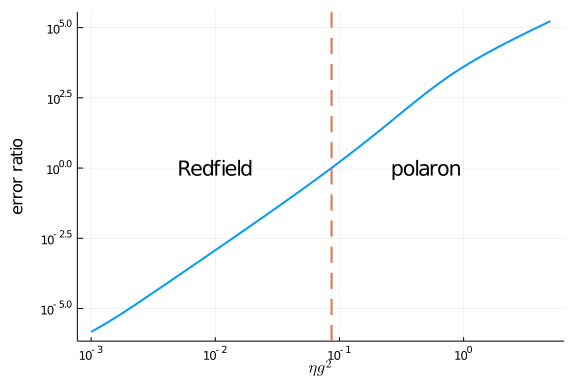
\includegraphics[width=\linewidth]{jl_u61kNo/02-polaron-transformed-redfield_1_1.pdf}

From above figure we can see that, as the system-bath coupling strength is bigger than $10^{-1}$, PTRE should have better error scaling than the usual form of Redfield equation.

\subsubsection{Solving PTRE}
Since PTRE and the Redfield equation have identical forms, \texttt{solve\_redfield} can also be used for PTRE. To see this, let's first write down the PTRE for our example.

\[
\dot{\rho}_\mathrm{S} = \epsilon \ensuremath{\sigma}_z + [ \sigma_i, \Lambda_i(t) \rho_\mathrm{S}(t) ] + h.c.
\]
where $i,j \in [+, -]$, $i \neq j$ and

\[
\Lambda_i(t)=\Delta^2 \int_0^{t} K(t-\tau)U(t,\tau) \sigma_j U^\dagger(t,\tau) \mathrm{d}\tau \ .
\]
From above equations, it is clear that the following steps are needed to define an annealing process in polaron frame:

\begin{itemize}
\item[1. ] define a new Hamiltonian $H = \epsilon \ensuremath{\sigma}_z$;


\item[2. ] define new coupling operators $\sigma_-$ and $\sigma_+$;


\item[3. ] define new correlated bath with two-point correlation $K_{i,j}(t_1, t_2)$;

\end{itemize}
The following code block illustrates how these can be done in OSQAT


\begin{lstlisting}
(*@\HLJLcs{{\#}}@*) (*@\HLJLcs{assume}@*) (*@\HLJLcs{\ensuremath{\epsilon}}@*) (*@\HLJLcs{=}@*) (*@\HLJLcs{1}@*)
    (*@\HLJLkd{const}@*) (*@\HLJLn{\ensuremath{\Delta}}@*) (*@\HLJLoB{=}@*) (*@\HLJLnfB{0.1}@*) 
    (*@\HLJLcs{{\#}}@*) (*@\HLJLcs{define}@*) (*@\HLJLcs{the}@*) (*@\HLJLcs{Ohmic}@*) (*@\HLJLcs{bath}@*) (*@\HLJLcs{in}@*) (*@\HLJLcs{polaron}@*) (*@\HLJLcs{transformed}@*) (*@\HLJLcs{frame}@*)
    (*@\HLJLn{\ensuremath{\eta}}@*) (*@\HLJLoB{=}@*) (*@\HLJLnfB{0.5}@*)(*@\HLJLp{;}@*) (*@\HLJLn{bath}@*) (*@\HLJLoB{=}@*) (*@\HLJLnf{Ohmic}@*)(*@\HLJLp{(}@*)(*@\HLJLn{\ensuremath{\eta}}@*)(*@\HLJLp{,}@*) (*@\HLJLn{fc}@*)(*@\HLJLp{,}@*) (*@\HLJLn{T}@*)(*@\HLJLp{)}@*)
    (*@\HLJLnf{K}@*)(*@\HLJLp{(}@*)(*@\HLJLn{t1}@*)(*@\HLJLp{,}@*) (*@\HLJLn{t2}@*)(*@\HLJLp{)}@*) (*@\HLJLoB{=}@*) (*@\HLJLn{\ensuremath{\Delta}}@*)(*@\HLJLoB{{\textasciicircum}}@*)(*@\HLJLni{2}@*) (*@\HLJLoB{*}@*) (*@\HLJLnf{polaron{\_}correlation}@*)(*@\HLJLp{(}@*)(*@\HLJLn{t1}@*)(*@\HLJLoB{-}@*)(*@\HLJLn{t2}@*)(*@\HLJLp{,}@*) (*@\HLJLn{bath}@*)(*@\HLJLp{)}@*)
    (*@\HLJLn{cfun}@*) (*@\HLJLoB{=}@*) (*@\HLJLp{[}@*)(*@\HLJLn{nothing}@*) (*@\HLJLn{K}@*)(*@\HLJLp{;}@*) (*@\HLJLn{K}@*) (*@\HLJLn{nothing}@*)(*@\HLJLp{]}@*)
    (*@\HLJLn{pbath}@*) (*@\HLJLoB{=}@*) (*@\HLJLnf{CorrelatedBath}@*)(*@\HLJLp{(((}@*)(*@\HLJLni{1}@*)(*@\HLJLp{,}@*)(*@\HLJLni{2}@*)(*@\HLJLp{),(}@*)(*@\HLJLni{2}@*)(*@\HLJLp{,}@*)(*@\HLJLni{1}@*)(*@\HLJLp{)),}@*) (*@\HLJLn{correlation}@*)(*@\HLJLoB{=}@*)(*@\HLJLn{cfun}@*)(*@\HLJLp{)}@*)
    (*@\HLJLcs{{\#}}@*) (*@\HLJLcs{define}@*) (*@\HLJLcs{coupling}@*) (*@\HLJLcs{as}@*) (*@\HLJLcs{\ensuremath{\sigma}+}@*) (*@\HLJLcs{and}@*) (*@\HLJLcs{\ensuremath{\sigma}-}@*) (*@\HLJLcs{operators}@*)
    (*@\HLJLn{\ensuremath{\sigma}p}@*) (*@\HLJLoB{=}@*) (*@\HLJLp{[}@*)(*@\HLJLni{0}@*) (*@\HLJLni{1}@*)(*@\HLJLp{;}@*)(*@\HLJLni{0}@*) (*@\HLJLnfB{0.0}@*)(*@\HLJLn{im}@*)(*@\HLJLp{];}@*) (*@\HLJLn{\ensuremath{\sigma}m}@*) (*@\HLJLoB{=}@*) (*@\HLJLp{[}@*)(*@\HLJLni{0}@*) (*@\HLJLni{0}@*)(*@\HLJLp{;}@*)(*@\HLJLni{1}@*) (*@\HLJLnfB{0.0}@*)(*@\HLJLn{im}@*)(*@\HLJLp{]}@*)
    (*@\HLJLn{coupling}@*) (*@\HLJLoB{=}@*) (*@\HLJLnf{ConstantCouplings}@*)(*@\HLJLp{([}@*)(*@\HLJLn{\ensuremath{\sigma}p}@*)(*@\HLJLp{,}@*) (*@\HLJLn{\ensuremath{\sigma}m}@*)(*@\HLJLp{])}@*)
    (*@\HLJLcs{{\#}}@*) (*@\HLJLcs{manually}@*) (*@\HLJLcs{define}@*) (*@\HLJLcs{the}@*) (*@\HLJLcs{unitary}@*) (*@\HLJLcs{operator}@*)
    (*@\HLJLnf{U}@*)(*@\HLJLp{(}@*)(*@\HLJLn{t}@*)(*@\HLJLp{)}@*) (*@\HLJLoB{=}@*) (*@\HLJLnf{exp}@*)(*@\HLJLp{(}@*)(*@\HLJLoB{-}@*)(*@\HLJLnfB{2.0}@*)(*@\HLJLn{im}@*) (*@\HLJLoB{*}@*) (*@\HLJLn{\ensuremath{\pi}}@*) (*@\HLJLoB{*}@*) (*@\HLJLn{\ensuremath{\sigma}z}@*) (*@\HLJLoB{*}@*) (*@\HLJLn{t}@*)(*@\HLJLp{)}@*)
    (*@\HLJLn{H}@*) (*@\HLJLoB{=}@*) (*@\HLJLnf{DenseHamiltonian}@*)(*@\HLJLp{([(}@*)(*@\HLJLn{s}@*)(*@\HLJLp{)}@*)(*@\HLJLoB{->}@*)(*@\HLJLnfB{1.0}@*)(*@\HLJLp{],}@*) (*@\HLJLp{[}@*)(*@\HLJLn{\ensuremath{\sigma}z}@*)(*@\HLJLp{])}@*)
    (*@\HLJLn{u0}@*) (*@\HLJLoB{=}@*) (*@\HLJLn{PauliVec}@*)(*@\HLJLp{[}@*)(*@\HLJLni{3}@*)(*@\HLJLp{][}@*)(*@\HLJLni{1}@*)(*@\HLJLp{]}@*)
    (*@\HLJLn{annealing}@*) (*@\HLJLoB{=}@*) (*@\HLJLnf{Annealing}@*)(*@\HLJLp{(}@*)(*@\HLJLn{H}@*)(*@\HLJLp{,}@*) (*@\HLJLn{u0}@*)(*@\HLJLp{,}@*) (*@\HLJLn{coupling}@*) (*@\HLJLoB{=}@*) (*@\HLJLn{coupling}@*)(*@\HLJLp{,}@*) (*@\HLJLn{bath}@*) (*@\HLJLoB{=}@*) (*@\HLJLn{pbath}@*)(*@\HLJLp{)}@*)
    (*@\HLJLn{tf}@*) (*@\HLJLoB{=}@*) (*@\HLJLni{100}@*)
    (*@\HLJLn{sol{\_}ptre}@*) (*@\HLJLoB{=}@*) (*@\HLJLnf{solve{\_}redfield}@*)(*@\HLJLp{(}@*)(*@\HLJLn{annealing}@*)(*@\HLJLp{,}@*) (*@\HLJLn{tf}@*)(*@\HLJLp{,}@*) (*@\HLJLn{U}@*)(*@\HLJLp{,}@*) (*@\HLJLn{alg}@*)(*@\HLJLoB{=}@*)(*@\HLJLnf{Tsit5}@*)(*@\HLJLp{(),}@*) (*@\HLJLn{Ta}@*)(*@\HLJLoB{=}@*)(*@\HLJLni{2}@*)(*@\HLJLp{,}@*) (*@\HLJLn{reltol}@*)(*@\HLJLoB{=}@*)(*@\HLJLnfB{1e-5}@*)(*@\HLJLp{)}@*)
    (*@\HLJLn{pop{\_}e}@*) (*@\HLJLoB{=}@*) (*@\HLJLp{[}@*)(*@\HLJLnf{real}@*)(*@\HLJLp{(}@*)(*@\HLJLn{s}@*)(*@\HLJLp{[}@*)(*@\HLJLni{1}@*)(*@\HLJLp{,}@*)(*@\HLJLni{1}@*)(*@\HLJLp{])}@*) (*@\HLJLk{for}@*) (*@\HLJLn{s}@*) (*@\HLJLkp{in}@*) (*@\HLJLn{sol{\_}ptre}@*)(*@\HLJLoB{.}@*)(*@\HLJLn{u}@*)(*@\HLJLp{]}@*)
    (*@\HLJLnf{plot}@*)(*@\HLJLp{(}@*)(*@\HLJLn{sol{\_}ptre}@*)(*@\HLJLoB{.}@*)(*@\HLJLn{t}@*)(*@\HLJLp{,}@*) (*@\HLJLn{pop{\_}e}@*)(*@\HLJLp{,}@*) (*@\HLJLn{xlabel}@*)(*@\HLJLoB{=}@*)(*@\HLJLso{L"{}t{\textbackslash}}@*) (*@\HLJLso{({\textbackslash}mathrm{\{}ns{\}})"{}}@*)(*@\HLJLp{,}@*) (*@\HLJLn{ylabel}@*)(*@\HLJLoB{=}@*)(*@\HLJLso{L"{}P{\_}0(t)"{}}@*)(*@\HLJLp{,}@*) (*@\HLJLn{label}@*)(*@\HLJLoB{=}@*)(*@\HLJLs{"{}"{}}@*)(*@\HLJLp{,}@*) (*@\HLJLn{linewidth}@*) (*@\HLJLoB{=}@*) (*@\HLJLni{2}@*)(*@\HLJLp{)}@*)
\end{lstlisting}

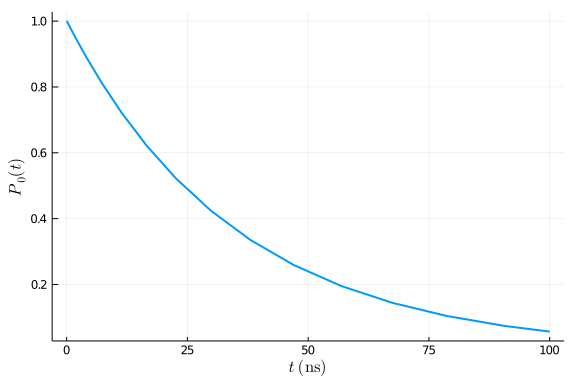
\includegraphics[width=\linewidth]{jl_u61kNo/02-polaron-transformed-redfield_2_1.pdf}

For historical reasons, this is know as an example of the "incoherent tunneling". The off-diagonal elements of the density matrix in computational bases(Z-bases) during the entire evolution is 0(, which is shown in next section).

\subsubsection{Redfield equation}
What would happend to normal Redfield equation in this regime? We can also try


\begin{lstlisting}
(*@\HLJLn{H}@*) (*@\HLJLoB{=}@*) (*@\HLJLnf{DenseHamiltonian}@*)(*@\HLJLp{([(}@*)(*@\HLJLn{s}@*)(*@\HLJLp{)}@*)(*@\HLJLoB{->}@*)(*@\HLJLnfB{1.0}@*)(*@\HLJLp{],}@*) (*@\HLJLp{[}@*)(*@\HLJLn{\ensuremath{\sigma}z}@*)(*@\HLJLoB{+}@*)(*@\HLJLnfB{0.1}@*)(*@\HLJLoB{*}@*)(*@\HLJLn{\ensuremath{\sigma}x}@*)(*@\HLJLp{])}@*)
(*@\HLJLn{coupling}@*) (*@\HLJLoB{=}@*) (*@\HLJLnf{ConstantCouplings}@*)(*@\HLJLp{([}@*)(*@\HLJLs{"{}Z"{}}@*)(*@\HLJLp{])}@*)
(*@\HLJLn{annealing}@*) (*@\HLJLoB{=}@*) (*@\HLJLnf{Annealing}@*)(*@\HLJLp{(}@*)(*@\HLJLn{H}@*)(*@\HLJLp{,}@*) (*@\HLJLn{u0}@*)(*@\HLJLp{,}@*) (*@\HLJLn{coupling}@*) (*@\HLJLoB{=}@*) (*@\HLJLn{coupling}@*)(*@\HLJLp{,}@*) (*@\HLJLn{bath}@*) (*@\HLJLoB{=}@*) (*@\HLJLn{bath}@*)(*@\HLJLp{)}@*)
(*@\HLJLn{tf}@*) (*@\HLJLoB{=}@*) (*@\HLJLni{100}@*)
(*@\HLJLn{sol{\_}redfield}@*) (*@\HLJLoB{=}@*) (*@\HLJLnf{solve{\_}redfield}@*)(*@\HLJLp{(}@*)(*@\HLJLn{annealing}@*)(*@\HLJLp{,}@*) (*@\HLJLn{tf}@*)(*@\HLJLp{,}@*) (*@\HLJLn{U}@*)(*@\HLJLp{,}@*) (*@\HLJLn{alg}@*)(*@\HLJLoB{=}@*)(*@\HLJLnf{Tsit5}@*)(*@\HLJLp{(),}@*) (*@\HLJLn{Ta}@*)(*@\HLJLoB{=}@*)(*@\HLJLni{40}@*)(*@\HLJLp{,}@*) (*@\HLJLn{reltol}@*)(*@\HLJLoB{=}@*)(*@\HLJLnfB{1e-5}@*)(*@\HLJLp{,}@*) (*@\HLJLn{callback}@*)(*@\HLJLoB{=}@*)(*@\HLJLnf{PositivityCheckCallback}@*)(*@\HLJLp{())}@*)
(*@\HLJLn{pop{\_}e{\_}redfield}@*) (*@\HLJLoB{=}@*) (*@\HLJLp{[}@*)(*@\HLJLnf{real}@*)(*@\HLJLp{(}@*)(*@\HLJLn{s}@*)(*@\HLJLp{[}@*)(*@\HLJLni{1}@*)(*@\HLJLp{,}@*)(*@\HLJLni{1}@*)(*@\HLJLp{])}@*) (*@\HLJLk{for}@*) (*@\HLJLn{s}@*) (*@\HLJLkp{in}@*) (*@\HLJLn{sol{\_}redfield}@*)(*@\HLJLoB{.}@*)(*@\HLJLn{u}@*)(*@\HLJLp{]}@*)
(*@\HLJLnf{plot}@*)(*@\HLJLp{(}@*)(*@\HLJLn{sol{\_}ptre}@*)(*@\HLJLoB{.}@*)(*@\HLJLn{t}@*)(*@\HLJLp{,}@*) (*@\HLJLn{pop{\_}e}@*)(*@\HLJLp{,}@*) (*@\HLJLn{xlabel}@*)(*@\HLJLoB{=}@*)(*@\HLJLso{L"{}t{\textbackslash}}@*) (*@\HLJLso{({\textbackslash}mathrm{\{}ns{\}})"{}}@*)(*@\HLJLp{,}@*) (*@\HLJLn{ylabel}@*)(*@\HLJLoB{=}@*)(*@\HLJLso{L"{}P{\_}0(t)"{}}@*)(*@\HLJLp{,}@*) (*@\HLJLn{label}@*)(*@\HLJLoB{=}@*)(*@\HLJLs{"{}PTRE"{}}@*)(*@\HLJLp{,}@*) (*@\HLJLn{linewidth}@*) (*@\HLJLoB{=}@*) (*@\HLJLni{2}@*)(*@\HLJLp{,}@*) (*@\HLJLn{legend}@*) (*@\HLJLoB{=}@*) (*@\HLJLsc{:right}@*)(*@\HLJLp{)}@*)
(*@\HLJLnf{plot!}@*)(*@\HLJLp{(}@*)(*@\HLJLn{sol{\_}redfield}@*)(*@\HLJLoB{.}@*)(*@\HLJLn{t}@*)(*@\HLJLp{,}@*) (*@\HLJLn{pop{\_}e{\_}redfield}@*)(*@\HLJLp{,}@*) (*@\HLJLn{xlabel}@*)(*@\HLJLoB{=}@*)(*@\HLJLso{L"{}t{\textbackslash}}@*) (*@\HLJLso{({\textbackslash}mathrm{\{}ns{\}})"{}}@*)(*@\HLJLp{,}@*) (*@\HLJLn{ylabel}@*)(*@\HLJLoB{=}@*)(*@\HLJLso{L"{}P{\_}0(t)"{}}@*)(*@\HLJLp{,}@*) (*@\HLJLn{label}@*)(*@\HLJLoB{=}@*)(*@\HLJLs{"{}Redfield"{}}@*)(*@\HLJLp{,}@*) (*@\HLJLn{linewidth}@*) (*@\HLJLoB{=}@*) (*@\HLJLni{2}@*)(*@\HLJLp{)}@*)
\end{lstlisting}

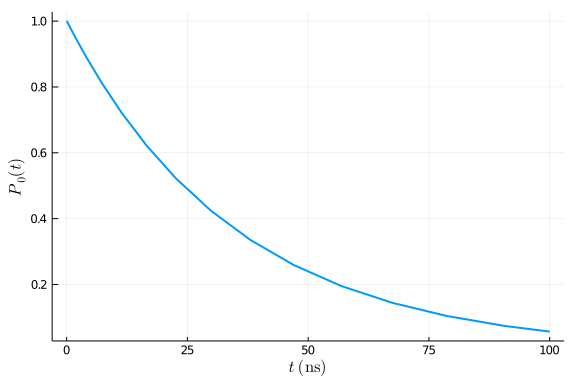
\includegraphics[width=\linewidth]{jl_u61kNo/02-polaron-transformed-redfield_3_1.pdf}

PTRE gives a much stronger decay than the Redfield equation for the parameters chosen in this example. One can also verify the amplitude of the off-diagonal elements during the evolution. Unlike PTRE, the usual Redfield equation have non-vanishing off-diagonal elements of the density matrix.


\begin{lstlisting}
(*@\HLJLn{t{\_}axis}@*) (*@\HLJLoB{=}@*) (*@\HLJLnf{range}@*)(*@\HLJLp{(}@*)(*@\HLJLni{0}@*)(*@\HLJLp{,}@*) (*@\HLJLni{5}@*)(*@\HLJLp{,}@*) (*@\HLJLn{length}@*)(*@\HLJLoB{=}@*)(*@\HLJLni{100}@*)(*@\HLJLp{)}@*)
(*@\HLJLn{off{\_}diag{\_}ptre}@*) (*@\HLJLoB{=}@*) (*@\HLJLp{[}@*)(*@\HLJLnf{abs}@*)(*@\HLJLp{(}@*)(*@\HLJLnf{sol{\_}ptre}@*)(*@\HLJLp{(}@*)(*@\HLJLn{t}@*)(*@\HLJLp{)[}@*)(*@\HLJLni{1}@*)(*@\HLJLp{,}@*)(*@\HLJLni{2}@*)(*@\HLJLp{])}@*) (*@\HLJLk{for}@*) (*@\HLJLn{t}@*) (*@\HLJLkp{in}@*) (*@\HLJLn{t{\_}axis}@*)(*@\HLJLp{]}@*)
(*@\HLJLn{off{\_}diag{\_}redfield}@*) (*@\HLJLoB{=}@*) (*@\HLJLp{[}@*)(*@\HLJLnf{abs}@*)(*@\HLJLp{(}@*)(*@\HLJLnf{sol{\_}redfield}@*)(*@\HLJLp{(}@*)(*@\HLJLn{t}@*)(*@\HLJLp{)[}@*)(*@\HLJLni{1}@*)(*@\HLJLp{,}@*)(*@\HLJLni{2}@*)(*@\HLJLp{])}@*) (*@\HLJLk{for}@*) (*@\HLJLn{t}@*) (*@\HLJLkp{in}@*) (*@\HLJLn{t{\_}axis}@*)(*@\HLJLp{]}@*)
(*@\HLJLnf{plot}@*)(*@\HLJLp{(}@*)(*@\HLJLn{t{\_}axis}@*)(*@\HLJLp{,}@*) (*@\HLJLn{off{\_}diag{\_}ptre}@*)(*@\HLJLp{,}@*) (*@\HLJLn{xlabel}@*)(*@\HLJLoB{=}@*)(*@\HLJLso{L"{}t{\textbackslash}}@*) (*@\HLJLso{({\textbackslash}mathrm{\{}ns{\}})"{}}@*)(*@\HLJLp{,}@*) (*@\HLJLn{ylabel}@*)(*@\HLJLoB{=}@*)(*@\HLJLso{L"{}{\textbackslash}lvert}@*) (*@\HLJLso{P{\_}{\{}12{\}}}@*) (*@\HLJLso{{\textbackslash}rvert|(t)"{}}@*)(*@\HLJLp{,}@*) (*@\HLJLn{label}@*)(*@\HLJLoB{=}@*)(*@\HLJLs{"{}PTRE"{}}@*)(*@\HLJLp{,}@*) (*@\HLJLn{linewidth}@*) (*@\HLJLoB{=}@*) (*@\HLJLni{2}@*)(*@\HLJLp{,}@*) (*@\HLJLn{legend}@*)(*@\HLJLoB{=:}@*)(*@\HLJLn{right}@*)(*@\HLJLp{)}@*)
(*@\HLJLnf{plot!}@*)(*@\HLJLp{(}@*)(*@\HLJLn{t{\_}axis}@*)(*@\HLJLp{,}@*) (*@\HLJLn{off{\_}diag{\_}redfield}@*)(*@\HLJLp{,}@*) (*@\HLJLn{xlabel}@*)(*@\HLJLoB{=}@*)(*@\HLJLso{L"{}t{\textbackslash}}@*) (*@\HLJLso{({\textbackslash}mathrm{\{}ns{\}})"{}}@*)(*@\HLJLp{,}@*) (*@\HLJLn{ylabel}@*)(*@\HLJLoB{=}@*)(*@\HLJLso{L"{}|P{\_}{\{}12{\}}(t)|"{}}@*)(*@\HLJLp{,}@*) (*@\HLJLn{label}@*)(*@\HLJLoB{=}@*)(*@\HLJLs{"{}Redfield"{}}@*)(*@\HLJLp{,}@*) (*@\HLJLn{linewidth}@*) (*@\HLJLoB{=}@*) (*@\HLJLni{2}@*)(*@\HLJLp{)}@*)
\end{lstlisting}

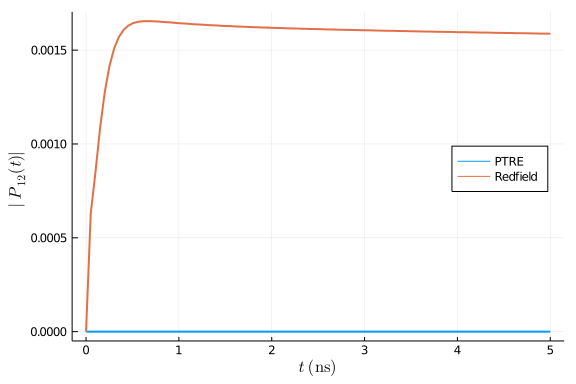
\includegraphics[width=\linewidth]{jl_u61kNo/02-polaron-transformed-redfield_4_1.pdf}


\end{document}
